% kapitel2.tex



\section{Hardware - Komponenten und Aufbau}
\label{chapter:kap1}
Der Spiegel besteht aus drei wesentlichen Komponenten: dem Spiegel, dem Monitor und der Steuereinheit, die alle darzustellenden Daten ermittelt. Diese Komponenten sind in Tabelle 1 aufgeführt und werden im Folgenden näher beschrieben. Während die erste Spalte die Komponente angibt, listet die zweite Spalte die Bauteile, sowie Arbeitsmaterial, im Detail auf. Spalte vier gibt die Bezugsquelle als Link an und die letzte Spalte enthält die Einkaufspreise.
\begin{table}[H]
	\scriptsize
	\begin{tabular}{R{2cm}|L{6.5cm}|L{2cm}|R{1.5cm}}
		& \textbf{Komponente} & \textbf{Link} & \textbf{Preis €} \\
		\hline
		\multirow{4}{2cm}{\textbf{Spiegel}} & IKEA RIBBA Rahmen, schwarz &
		\href{http://www.ikea.com/de/de/catalog/products/00078051/#/20078050}{IKEA} & 12,99 \\
		& Spionspiegelfolie & \href{https://www.amazon.de/Fenster-Spiegelfolie-Sichtschutzfolie-Fensterfolie-Selbstklebend/dp/B010677IAG/ref=sr_1_2?s=kitchen&ie=UTF8&qid=1503392562&sr=1-2&keywords=spionspiegelfolie}{Amazon} & 13,89 \\
		& Climapor Dämmplatte PUR & \href{https://www.bauhaus.info/isolierplatten-daemmung/daemmplatte-alu-kas08mx06x10mm-pur/p/15230648}{Bauhaus} & 12,95 \\
		& Dupli-Color COLOR Schwarz Matt Acryllackspray  & \href{https://www.bauhaus.info/buntlackspray/deco-matt-schwarz-150-ml-duplicolor/p/15073283?q=Sprühlack schwarz matt}{Bauhaus} & 5,50 \\
		\hline
		\multirow{4}{2cm}{\textbf{Monitor}} & 17' Monitor Acer TFT V176Lbmd & \href{https://www.bueromarkt-ag.de/monitor_acer_tft_v176lbmd,p-ac-v176l,h-acer.html"}
				{Büromarkt Böttcher} & 142,79 \\ 
		& Monitornetzteil* & -- & -- \\
		& Display Controller VGA zu IPEX-40Pin LVDS Kabel* & -- & -- \\
		& HDMI zu VGA Adapter & \href{https://www.amazon.de/Splaks-Vergoldete-Konverter-Audio-\%C3\%9Cbertragung-Chromebook/dp/B01IENVA6C/ref=sr_1_2?ie=UTF8&qid=1503391973&sr=8-2&keywords=hdmi+zu+vga+adapter+raspberry+pi}{Amazon} & 6,49 \\
		\hline
		\multirow{5}{2cm}{\textbf{{Steuereinheit \newline und Sensoren}}} & Raspberry Pi 3 Modell B mit 1,2 GHz QuadCore CPU 
		& \href{https://www.rasppishop.de/Raspberry-Pi-3-Modell-B-mit-12-GHz-QuadCore-64Bit-CPU}{Raspishop} & 36,49 \\
		& Speicherkarte Sandisk microSDHC 16GB & \href{https://www.rasppishop.de/Sandisk-microSDHC-16GB-Class10-mit-Noobs}{Raspishop} & 11,49 \\
		& PIR Infrarot Bewegungssensor HC-SR501 & \href{https://www.rasppishop.de/PIR-Infrarot-Bewegungssensor-PIR-Sensor-HC-SR501}{Raspishop} & 3.99 \\
		& DHT11 Digitaler Temperatur- und Feuchtigkeitssensor & \href{https://eckstein-shop.de/DHT11-Digitaler-Temperatur-und-Feuchtigkeitssensor-Modul-Arduino-Raspberry-Pi?curr=EUR&gclid=CjwKCAjwrO_MBRBxEiwAYJnDLPtR_FEgx77poEof21av-S9jQqb-Xs3GR1FSYe-mHwi6V57np8667hoCk74QAvD_BwE}{ECKSTEIN} & 4,48 \\
		& Anker Netzteil 24W 2x2,4A & \href{https://www.amazon.de/Anker-Ladeger\%C3\%A4t-PowerIQ-Technologie-Motorola/dp/B00WLI5E3M/ref=sr_1_2?ie=UTF8&qid=1503393782&sr=8-2&keywords=netzteil+2a}{Amazon} & 11,99 \\
	\end{tabular}
	\normalsize
\caption{Liste der Hardwarekomponenten}
$ ^{\textrm{*Bestandteil des Monitors}} $
\end{table}
Die Gesamtkosten belaufen sich somit auf \EUR{263,05}, jedoch ist dabei zu sagen, dass die Kosten stark Schwanken können, je nach dem welche Bauteile und Materialien für die Fertigung eingesetzt werden. So kann beispielsweise die Verwendung vorhandener Bauteile, z.B. eines alten Monitors, die Kosten entscheidend senken. Andererseits kann die Verwendung höherwertige Bauteile, z.B eines Full-HD Monitors oder eines professionellen Spionspiegels, den Preis deutlich steigern. Die Notwendigkeit das Display und die Steuereinheit hinter dem Spiegel unterzubringen impliziert eine Mindestgröße des Spiegels.

\subsection{Spiegel}
Als Spiegel kann entweder eine Einzelanfertigung in Eigenarbeit oder als Auftragsfertigung 
verwendet oder aber auf ein Fertig- oder Halbfertigprodukt zurückgegriffen werden. Während eine Einzelanfertigung eine hohe Flexibilität mit mehr Zeitaufwand und/oder höheren Kosten verbindet, erlaubt der Einsatz eines Halbfertigproduktes Flexibilität, Zeitaufwand und Kosten besser auszubalancieren. Aus diesen Gründen wird für das hier beschriebene Projekt auf Halbfertigprodukte zurückgegriffen. Konkret auf einen Bilderrahmen und eine Spiegelfolie.

\subsubsection*{Bilderrahmen}
Als Basis des Spiegels wird der IKEA-Bilderrahmen RIBBA mit einer Größe von50 x 50 x 4,5 cm verwendet. Bedauerlicherweise stehen auf Grund der Rückwand effektiv nur 4cm der Höhe zur Verfügung. Die Rückwand ist in den Rahmen integriert und raubt somit kostbaren Platz. Die verbleibende Herausforderung besteht darin, die restlichen Komponenten in der begrenzten Höhe unterzubringen, was jedoch bei einer geeigneten Platzierung der Komponenten sehr gut gelingt. 

\subsubsection*{Spiegelfolie}
Die Spiegelfolie für diesen Einsatzbereich muss besondere Anforderungen erfüllen. 
\begin{wrapfigure}{r}{0.5\textwidth}
	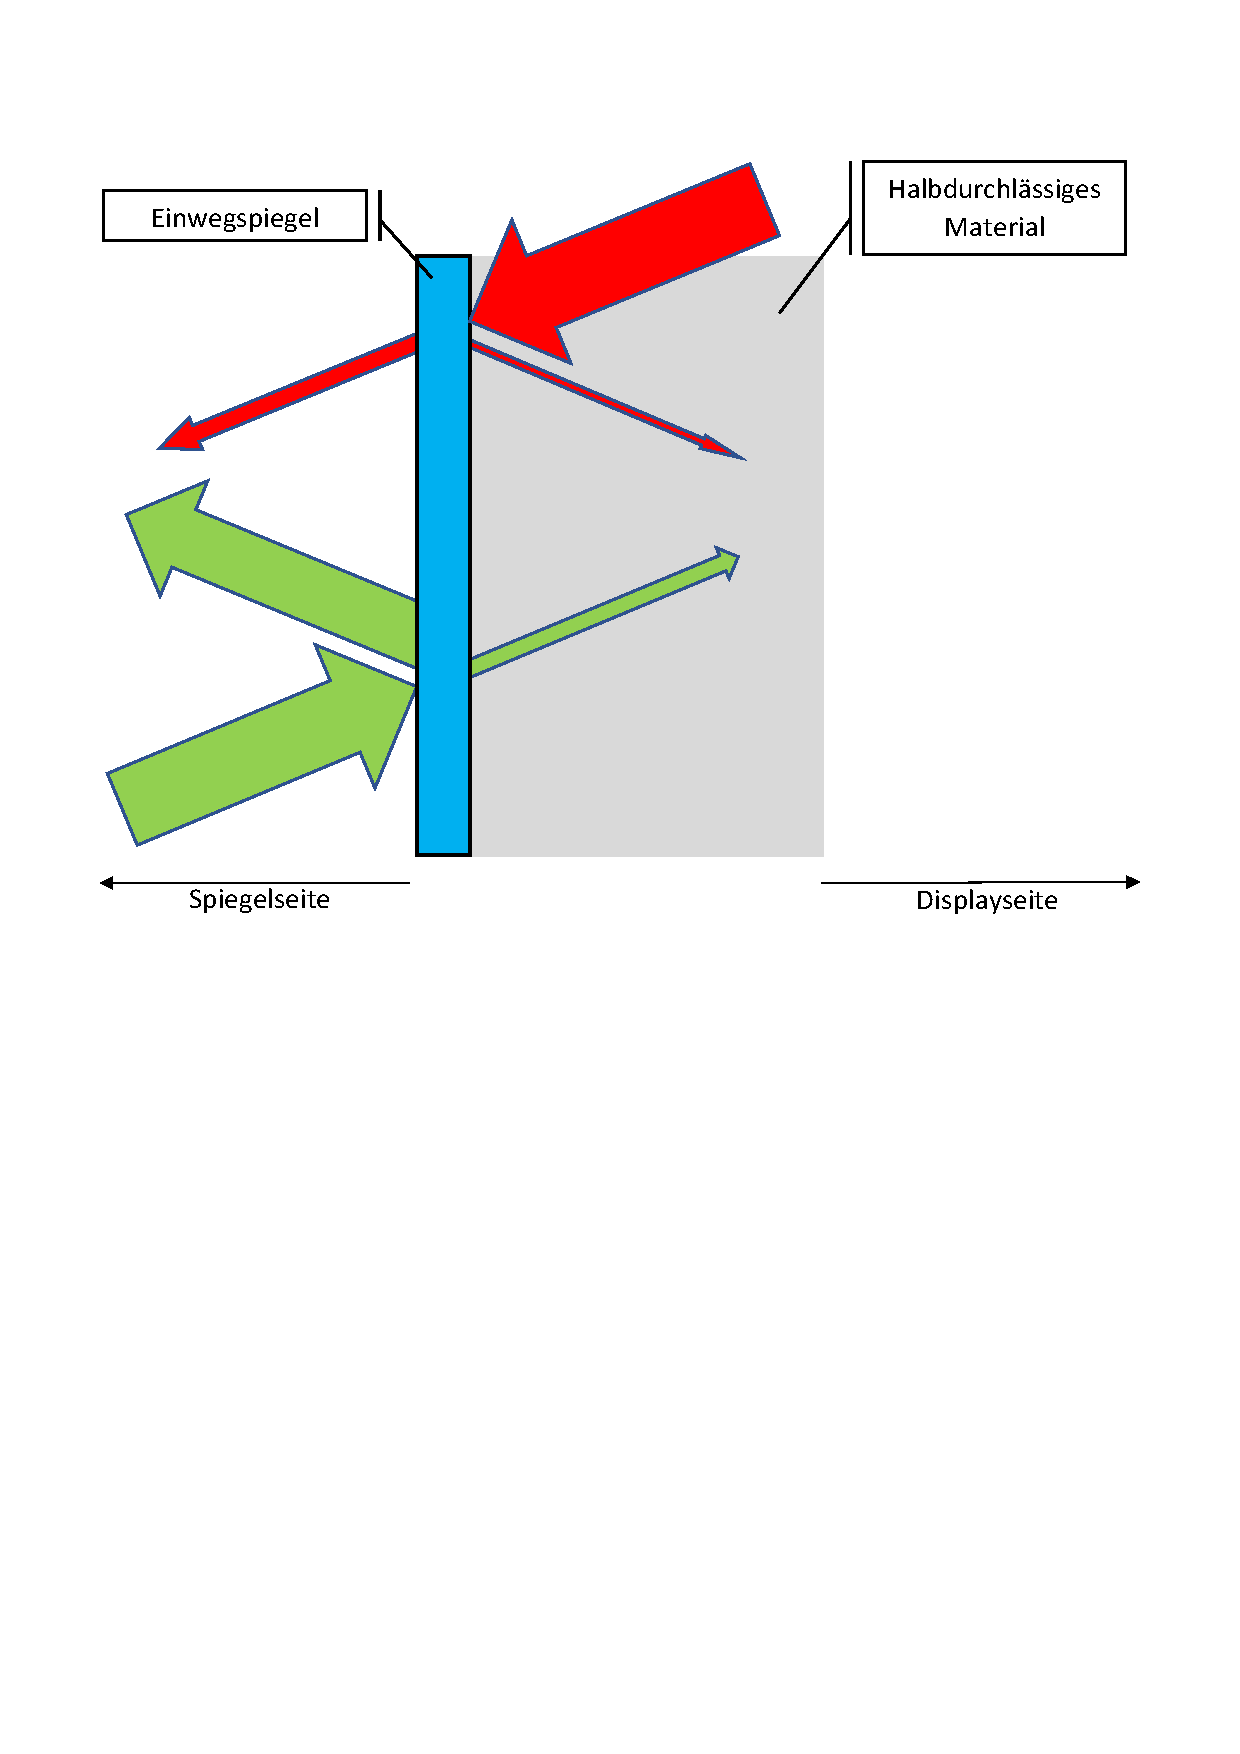
\includegraphics[trim=10mm 140mm 30mm 80mm, scale=0.35]{bilder/Einwegspiegel.pdf}
	\caption{Reflexions- und Transmissionswirkung}
\end{wrapfigure}
Sie muss einerseits für den Spiegeleffekt reflektierend sein, gleichzeitig aber auch lichtdurchlässig (transmissiv) sein, damit die Anzeige des Bildschirms hindurch scheinen kann. 

Spiegel oder Folien mit diesen Eigenschaften heißen Spionspiegel(-folien) bzw. Einwegspiegel. Entscheidend für die Qualität der Anzeige ist das Verhältnis zwischen dem Reflexionsgrad und der Transmission (vgl. Abbildung 2). Der rote Pfeil in der symbolisiert das Displaylicht und der grüne Pfeil das Umgebungslicht des Spiegels. Das Umgebungslicht wird zum größten Teil wieder reflektiert und das Displaylicht wird nahezu nach außen geleitet. Daher empfiehlt es sich einen Spiegel mit dem Reflexionsgrad von ca. 70-80\% und einem Transmissionswert von etwa 8\% zu verwenden. 


\subsubsection*{Folierung}
Die Folierung sollte in einem möglichst staubarmen Raum durchgeführt werden. Dabei wird 
ein Folienrakel oder eine Kreditkarte, eine Sprühflasche mit einer Wasser-Spülmittellösung (alternativ Scheibenreiniger), ein Cuttermesser und ein Scheibentuch bzw. Microfasertuch, was am besten keine Fuseln hinterlässt, als Hilfsmittel benötigt.
%\begin{figure}
%	\begin{center}
%		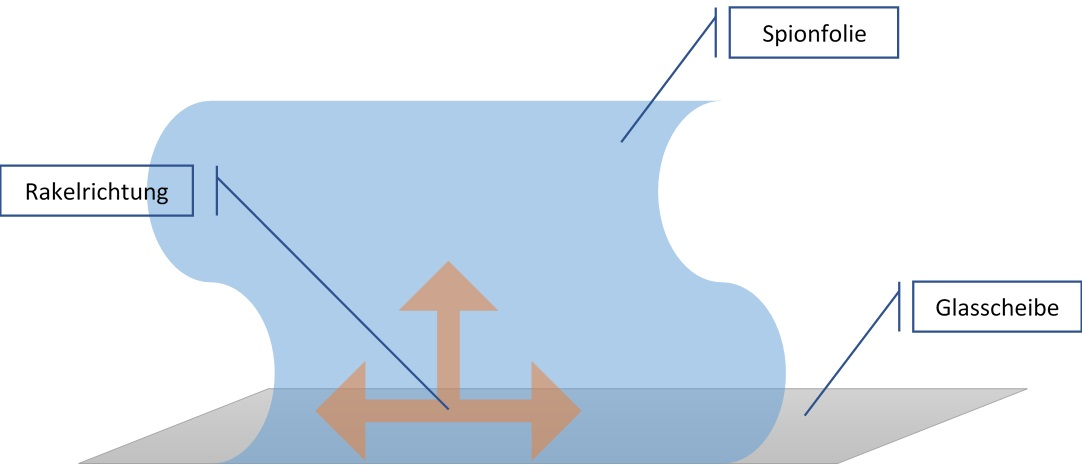
\includegraphics[scale=0.5]{bilder/Rakelanleitung.jpg}
%	\end{center}
%	\caption{Rakelrichtung}
%	\vspace{-10pt}
%\end{figure} 
Die Folie sollte idealerweise einige Zentimeter breiter und länger sein, als die Glasscheibe selbst, da Überstände im Nachgang mit dem Cuttermesser entfernt werden können. Die gründlich gereinigte Glasscheibe wird leicht mit dem Spülwasser befeuchtet, um eine Art Gleitschicht zu erzeugen. Nach Entfernung der Schutzschicht (falls vorhanden), wird die Folie auf die Glasscheibe aufgelegt. Vorhandene Luftbläschen werden mit Hilfe des Folienrakels heraus gestrichen (vgl. Abbildung 3). Ist das Ergebnis zufriedenstellend, sollte die Scheibe einen Tag liegen gelassen werden, bevor diese gereinigt und eingesetzt werden kann. Die Folierung erfordert selbst bei geringer Erfahrung nicht mehr als 15 Minuten. 

\begin{wrapfigure}{r}{0.45\textwidth}
		\includegraphics[scale=0.05]{bilder/spionspiegel.jpg}
		\caption{Folierung während des Proseminars}
\end{wrapfigure}
Durch die Verwendung einer Spionspiegelfolie kann zwar eine akzeptable Qualität erzielt werden. Bessere Ergebnisse erfordern jedoch eine professionell beschichtete Glasscheibe wie beispielsweise von der Firma Glas Star aus Bochum, die sich auf die Herstellung von Glasscheiben für Smart Mirrors spezialisiert hat (vgl. \href{https://www.glas-star.de/spionspiegelnachmass/chrome-spy-spiegel/}{Link}). 	
	





\subsection{Monitor}
Um dem Benutzer alle gesammelten Daten anzeigen zulassen, wird ein Monitor benötigt. Der Monitor kann entweder als fertiges Produkt (mit oder ohne Gehäuse) eingebaut oder aus einem Display, einem Display Controller und einem Netzteil zusammengebaut werden. Im zweiten Fall ist die Kompatibilität der Komponenten zu berücksichtigen. Bei der Wahl des Displays sind neben den Kosten vor allem die Auflösung und die Stromversorgung entscheidend. Ebenfalls relevant ist der Schwarzwert des Displays, da ein hoher Schwarzwert für ein geringes Durchscheinen des Bildschirmhintergrundes sorgt. Zu empfehlen sind hier OLED Displays, die einen höheren Schwarzwert aufweisen als beispielsweise LCD Displays.  
\begin{figure}[H]
	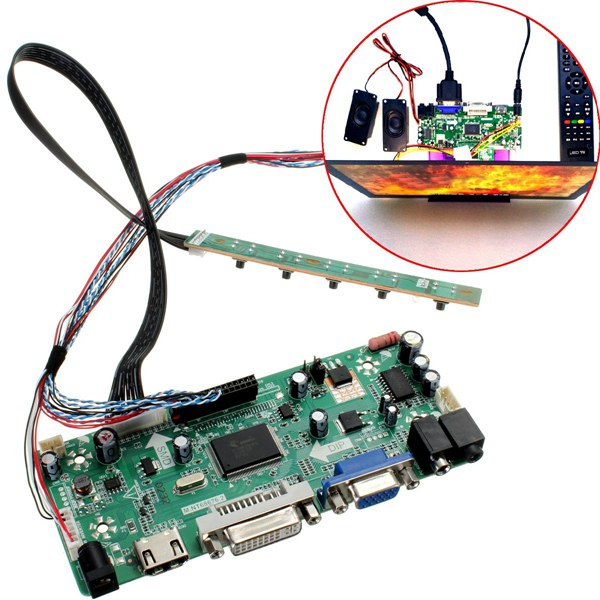
\includegraphics[trim=0mm 0mm 0mm 0mm, scale=1]{bilder/dcontroller.jpg}
	\caption{LCD Controller Board 40P}
\end{figure}
Für das vorliegende Projekt wurde ein Acer V176Lbmd Monitor mit einer Diagonale von 17' (ohne Gehäuse)verwendet. Der Monitor ist mit einem DVI und VGA Anschluss ausgestattet. Der Display Controller wandelt das Ausgangssignal der Steuereinheit um und leitet die Informationen über einen 40 Pin LVDS Anschluss an das Display weiter (Abbildung 9). Der Display Controller besitzen lediglich einen VGA Anschluss, so dass bei einem HDMI Ausgang an der Steuereinheit ein HDMI zu VGA Adapter zur Übermittlung des Displaysignals benötigt wird.
 

\subsection{Steuereinheit und Sensoren}
Der \textit{SmartMirror} benötigt eine Steuereinheit zum Sammeln und Aufbereiten der anzuzeigenden Daten. Diese Daten werden alternativ über das Internet oder über Sensoren zusammen getragen. Neben einem Internetzugang werden somit auch Sensoren, konkret ein Bewegungssensor, sowie ein Temperatur- und Luftfeuchtigkeitssensor, benötigt.

\subsubsection*{Raspberry Pi 3}
\begin{figure}[H]
	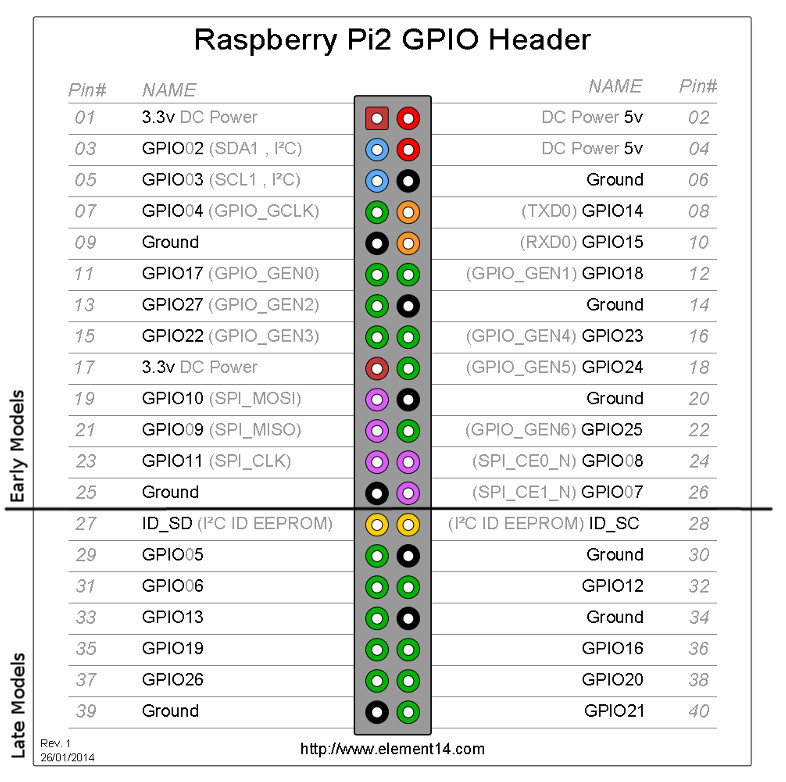
\includegraphics[scale=0.4]{bilder/gpio_pinout.jpg}
	\caption{GPIO-Belegung}
\end{figure}
Als Steuereinheit und Herzstück des \textit{SmartMirrors} dient ein Raspberry Pi 3 Model B. Das integrierte WLAN-Modul ermöglicht den mobilen Einsatz des \textit{SmartMirrors}, so dass dieser nicht fest an einen Ort gebunden ist. Für das Projekt werden lediglich einige der 40 GPIO-Anschlüsse des Boards für die Sensoren benötigt. Die genau Belegung der GPIO-Anschlüsse ist in Abbildung 5 grafisch dargestellt.

Unter dem Link \url{https://www.raspberrypi.org/documentation/} ist eine ausführliche Dokumentation zu den Eigenschaften des Raspberry Pi zu finden. Da der Raspberry Pi üblicherweise ohne ein Betriebssystem geliefert wird, wird unter der bereits genannten Adresse ebenfalls eine detaillierte Betriebssystem-Installationsanleitung bereit gestellt. Für das Projekt wird als Betriebssystem die ,,RASPBIAN JESSIE WITH DESKTOP`` Distribution verwendet. Alternativ zur Desktop Version gibt es auch eine Light Version. Diese ist wegen der fehlenden grafischen Oberfläche für dieses Projekt ungeeignet.

\subsubsection*{Bewegungssensor}
Der Bewegungssensor wird eingesetzt, um je nach Bedarf das Display ein- und auszuschalten und somit Energie zu sparen. Betritt eine Person den Raum, indem der Spiegel hängt, soll  der Sensor ein Signal zum Einschalten des Displays geben. Andernfalls bleibt das Display ausgeschaltet. 

	\begin{wrapfigure}{l}{0.4\textwidth}
		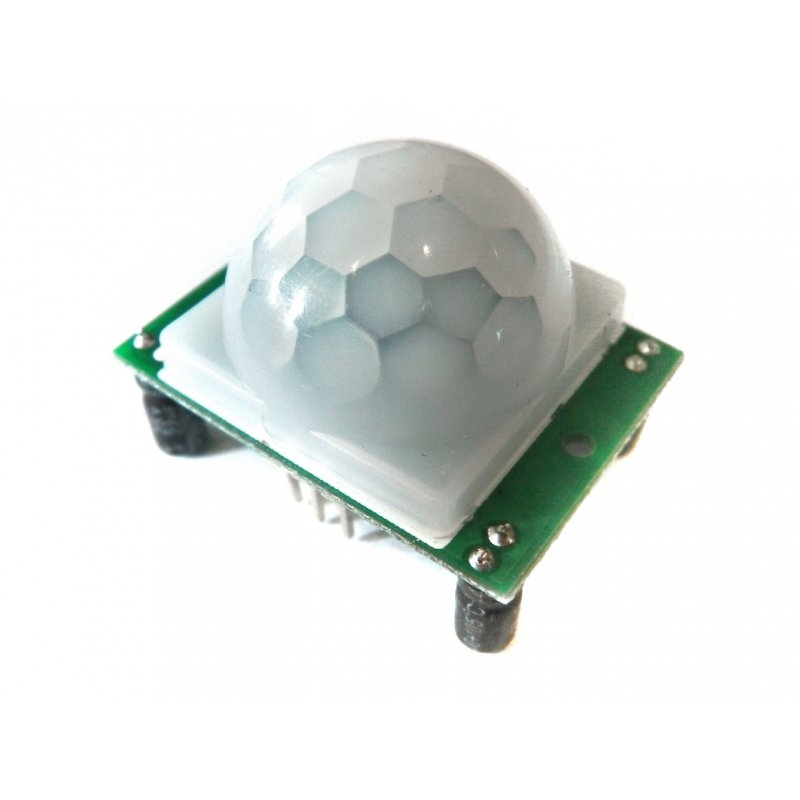
\includegraphics[width=0.9\textwidth]{bilder/PIR-Sensor.jpg}
		\caption{PIR-Sensor HC-SR501}
	\end{wrapfigure}	
Als Bewegungssensor für diesen Zweck ist das Modell HC-SR501 sehr gut geeignet. Der PIR-Sensor oder auch ,,IR-Bewegungssensor`` arbeitet passiv auf Basis der Infrarotstrahlung der Umgebung. Jeder Körper sendet eine kleine Menge an Infrarotstrahlung aus. Der PIR-Sensor stellt die Temperaturänderung im Raum fest und kann somit als Schalter verwendet werden. Der Sensor befindet sich auf einer kleinen Platine, besitzt eine einstellbare Empfindlichkeit und zwei M2 Befestigungsbohrungen für die Montage. Die Reichweite der Erfassung beträgt bis zu 7 Meter. Der Erfassungswinkel des Objektives beträgt etwa 100 Grad. 

Zum Anschließen des Sensors an den Raspberry Pi 3 werden zusätzlich drei Jumperkabel benötigt (VCC an Pin 2 (5V); OUT an Pin 16 (GPIO 23); GND an Pin 6 (Ground)). Alternativ dazu kann ein dreiadriges Kabel verwendet werden.

\subsubsection*{Temperatur- und Luftfeuchtigkeitssensor}
Der Temperatur- und Luftfeuchtigkeitssensor liefert Daten über den Raum, in dem der Spiegel hängt. Dazu ist der Sensor lediglich an das Raspberry Pi Board anzuschließen.
%\begin{figure}[H]
%	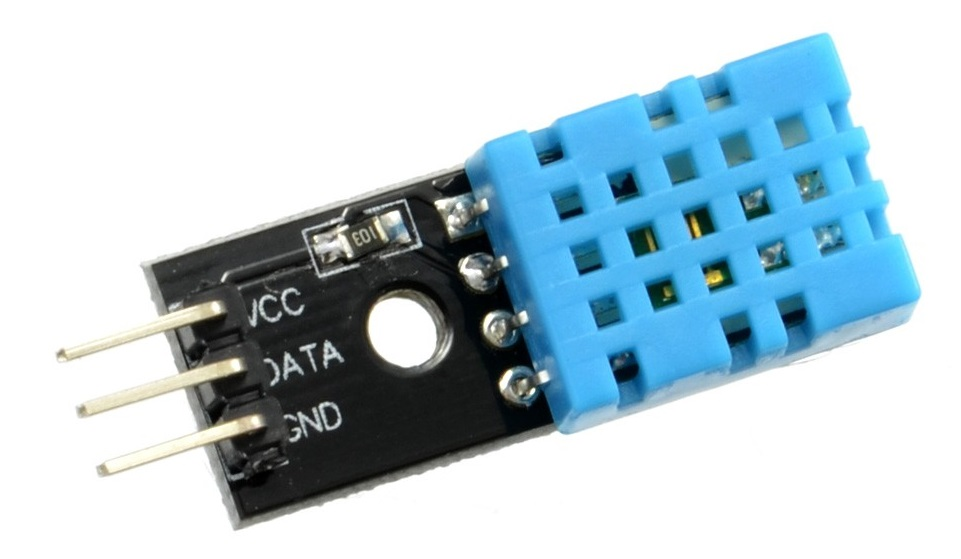
\includegraphics[trim=0mm 0mm 0mm 0mm, scale=0.3]{bilder/DHT11.jpg}
%	\caption{TL-Sensor DHT11}
%\end{figure}
 Der linke Pin (VCC) des Sensors wird an den Pin1 (3.3V) des Pi´s angeschlossen. Der mittlere Sensor Pin (DATA)  ermöglicht den Datenaustausch und wird mit einen freien GPIO Pin des Raspberry Pi´s (z.B. Pin7) verbunden. 
\begin{figure}[H]
	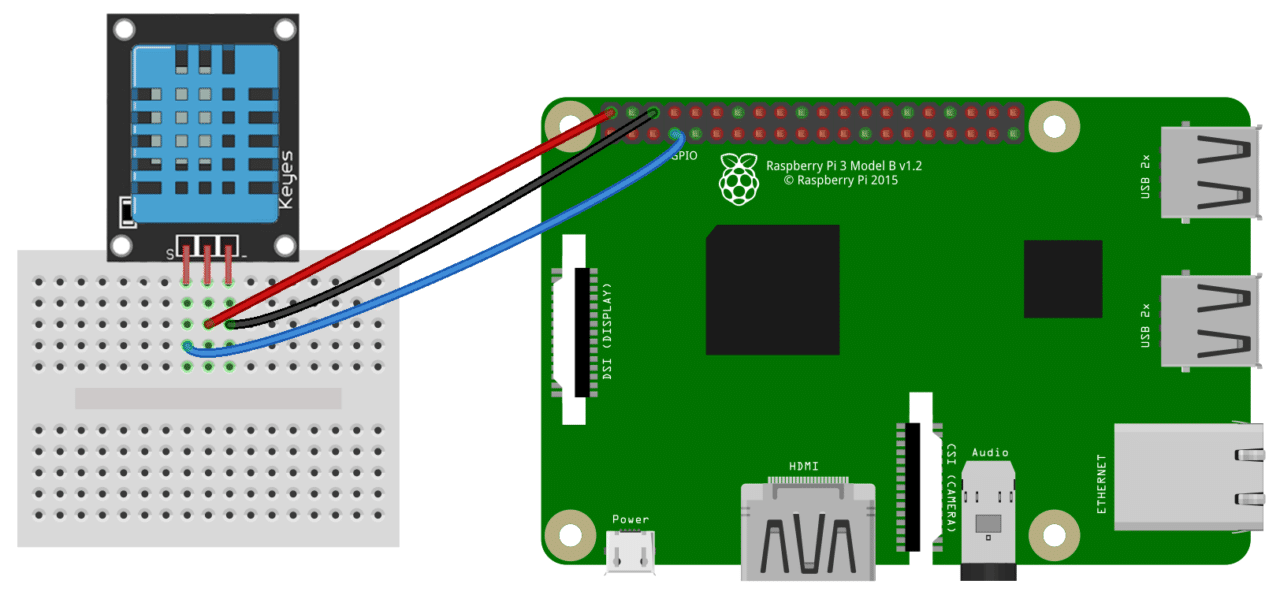
\includegraphics[trim=0mm 0mm 0mm 0mm, scale=1]{bilder/DHT11-on-the-Raspberry-Pi.png}
	\caption{DHT11 angeschlossen an ein Raspberry Pi}
\end{figure}
Der rechte Sensor Pin (GND) muss mit einem der Ground Pin´s (z.B. Pin5) des Raspberry Pi´s verbunden werden. Die Abbildung 8 illustriert den Anschluss des Sensors an ein Raspberry Pi bei Verwendung einer Steckplatine. Anzumerken ist, dass der linke und mittlere Anschluss in der Abbildung vertauscht sind.

\subsection{Aufbau}
Die Abbildung 10 zeigt einen Überblick über die Anordnung und Platzierung der verbauten Komponenten. 
\begin{figure}
	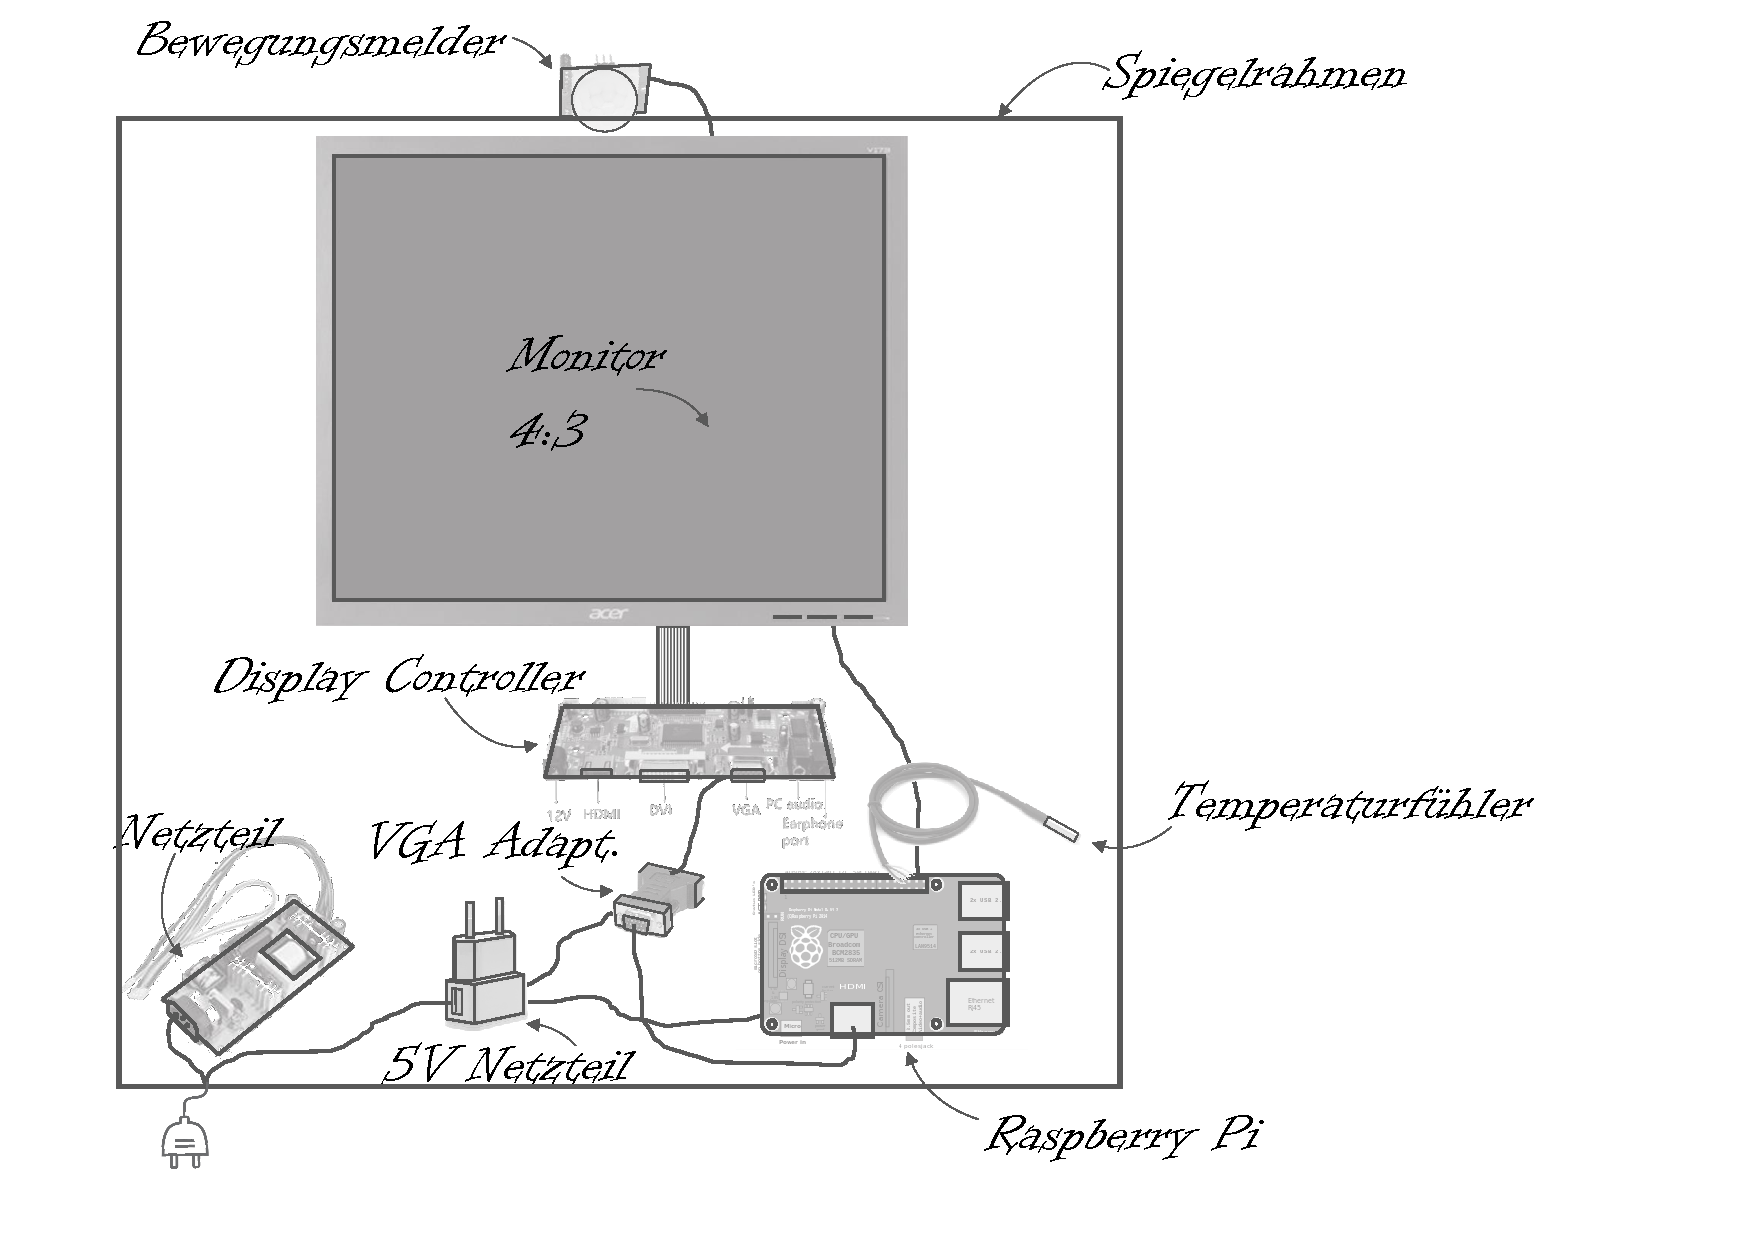
\includegraphics[scale=0.5, trim=0mm 10mm 60mm 10mm]{bilder/smartMirrorExplosionsskizze.pdf}
	\caption{Konstruktionsskizze}
\end{figure}
Da der Monitor den meisten Platz erfordert, müssen die übrigen Komponenten um das Display herum untergebracht werden. Es ist zu berücksichtigen, dass der Monitor mit  minimalem Abstand zur oberen Kante des Rahmens verbaut wird, damit der Spiegel je nach Form nicht zu weit nach oben gehangen werden muss. Zur Verbesserung des Halts der Komponenten, wird eine Hartschaumplatte eingesetzt. 

\begin{wrapfigure}{r}{0.45\textwidth}
	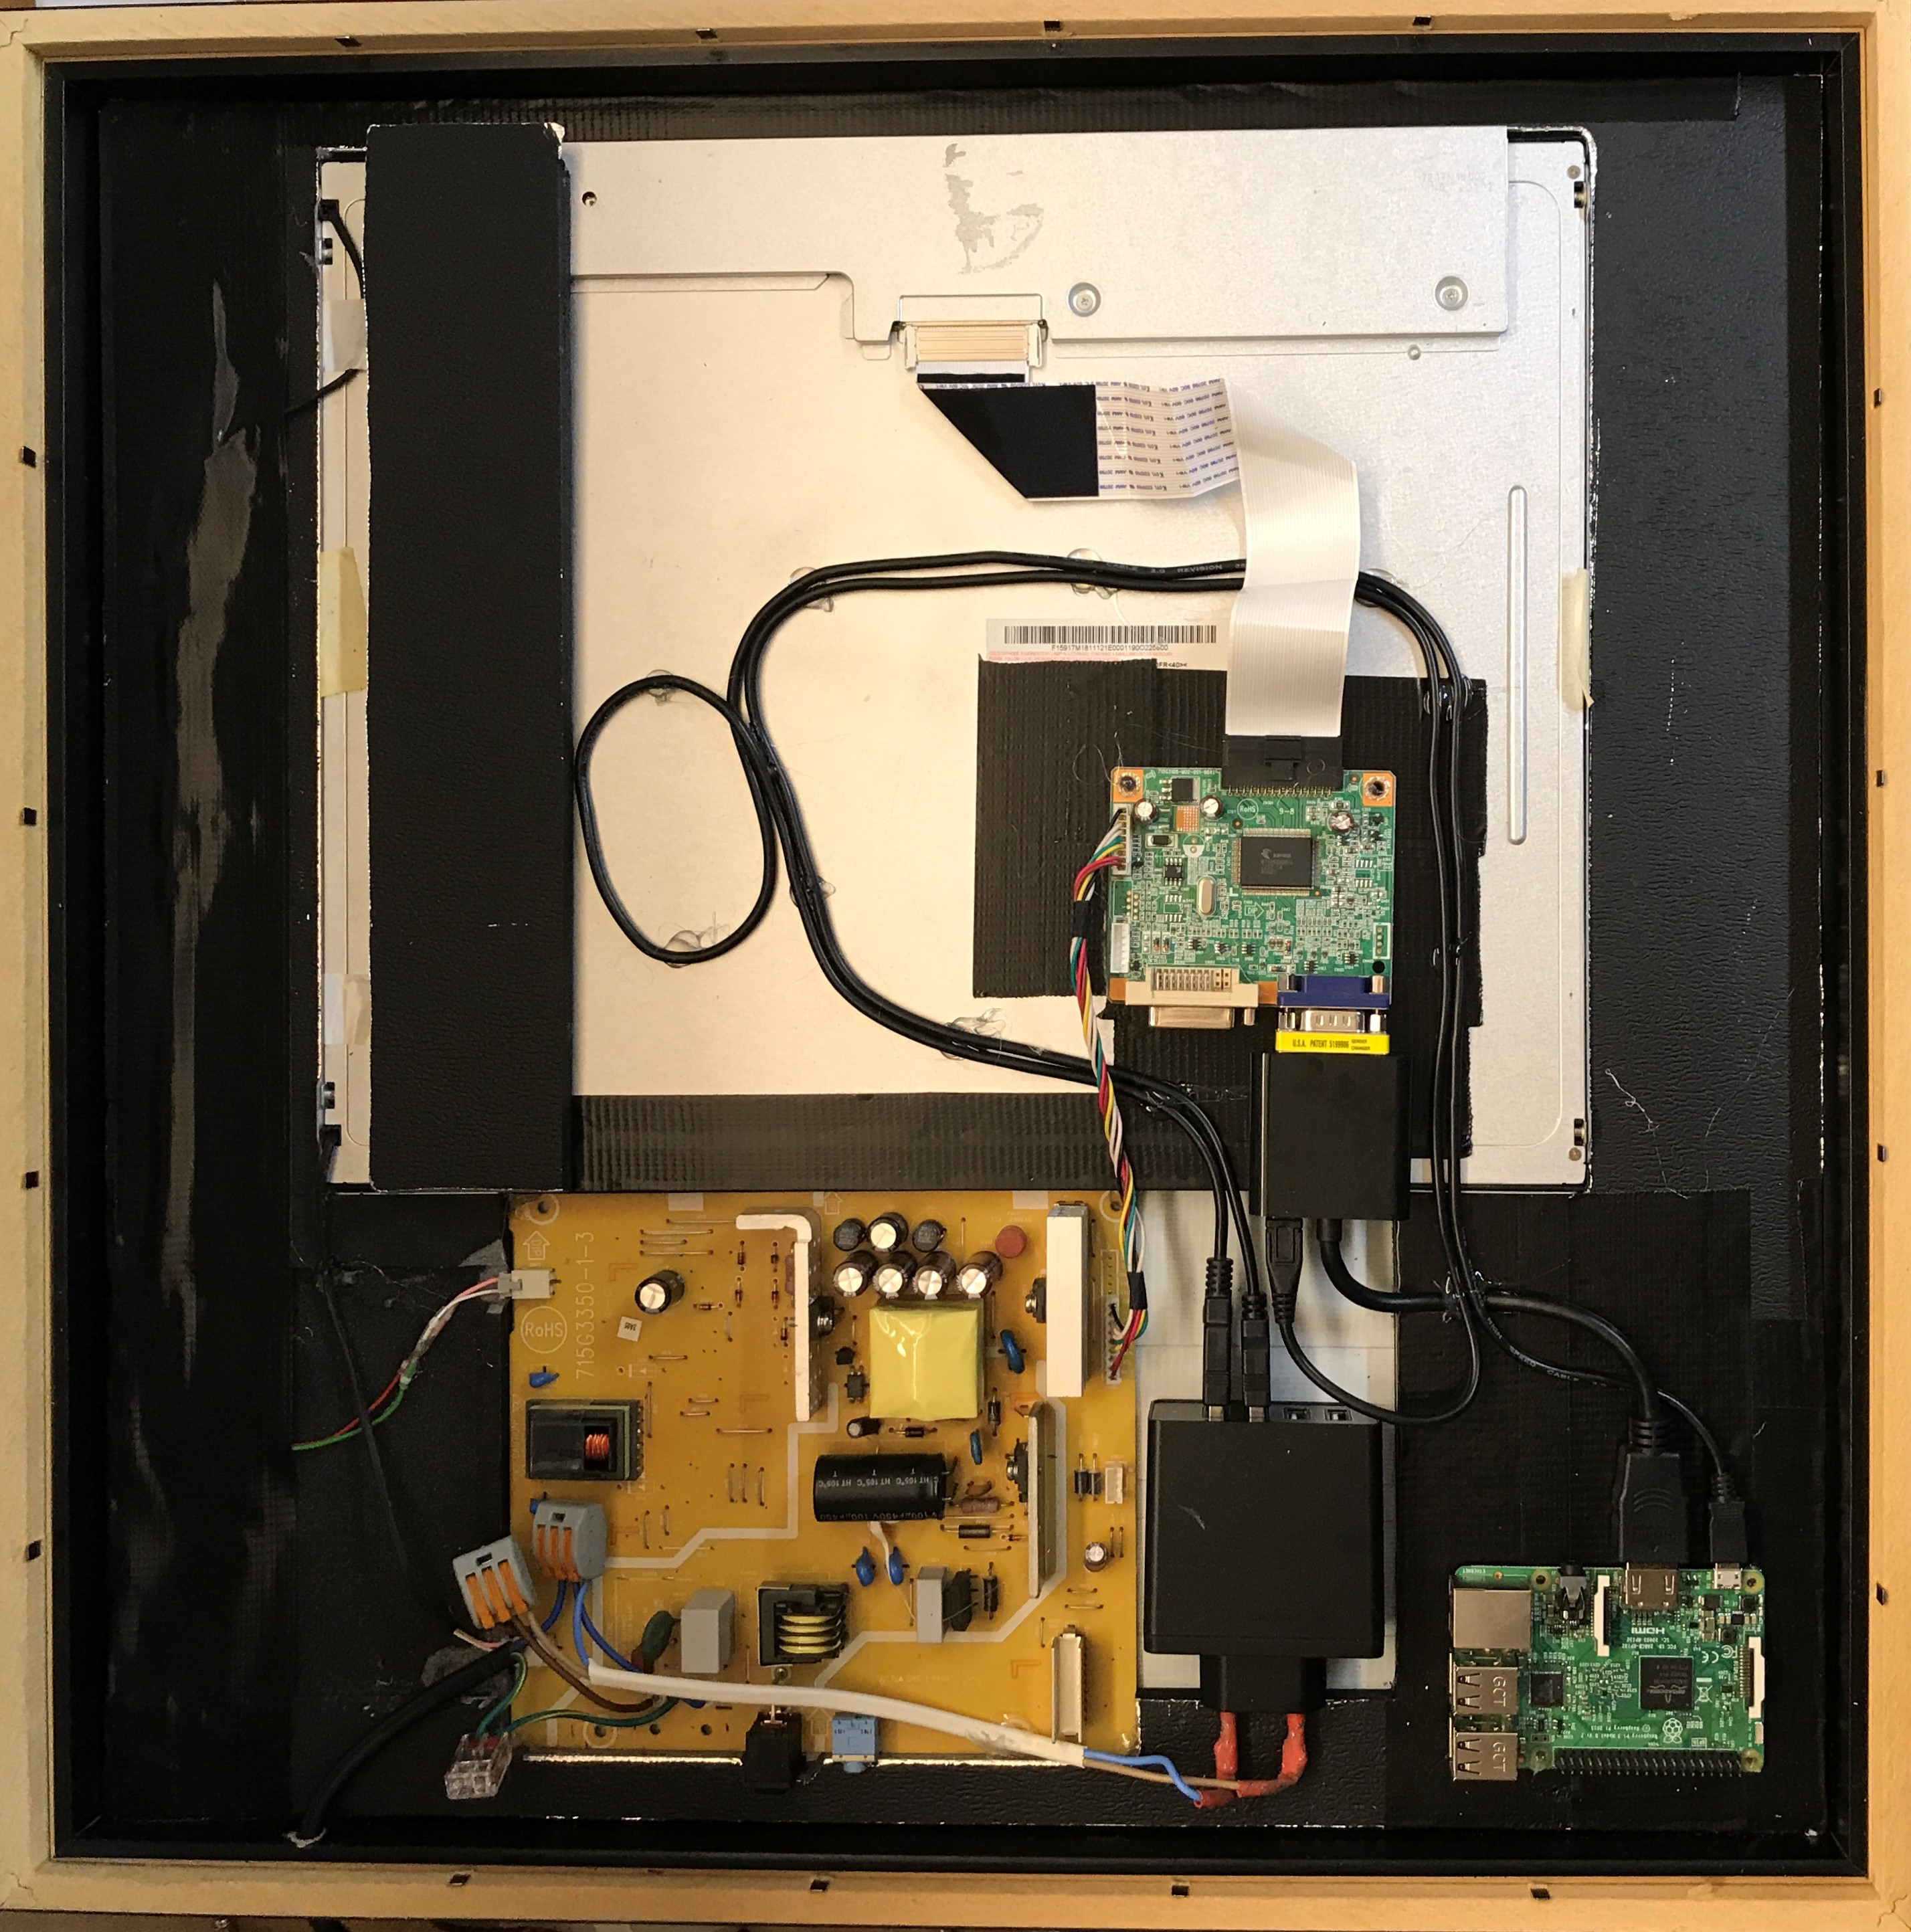
\includegraphics[scale=0.06]{bilder/Innenansicht.jpg}
	\caption{Anordnung und Verkabelung der Komponenten}
\end{wrapfigure}
Dazu wird ein Loch passend zur Größe des Displays ausgeschnitten und die anderen Komponenten auf der Platte platziert. Die Hartschaumplatte und die Rückwand sind für ein besseres Ergebnis des Spionspiegels von innen schwarz lackiert (Abbildung 12-13). 
Die dunkle Farbe absorbiert das eintretende Licht und vermindert die Reflexion. Ein Abbild der Rückseite wird in Abbildung 11 repräsentiert.

%\begin{figure}[H]
%	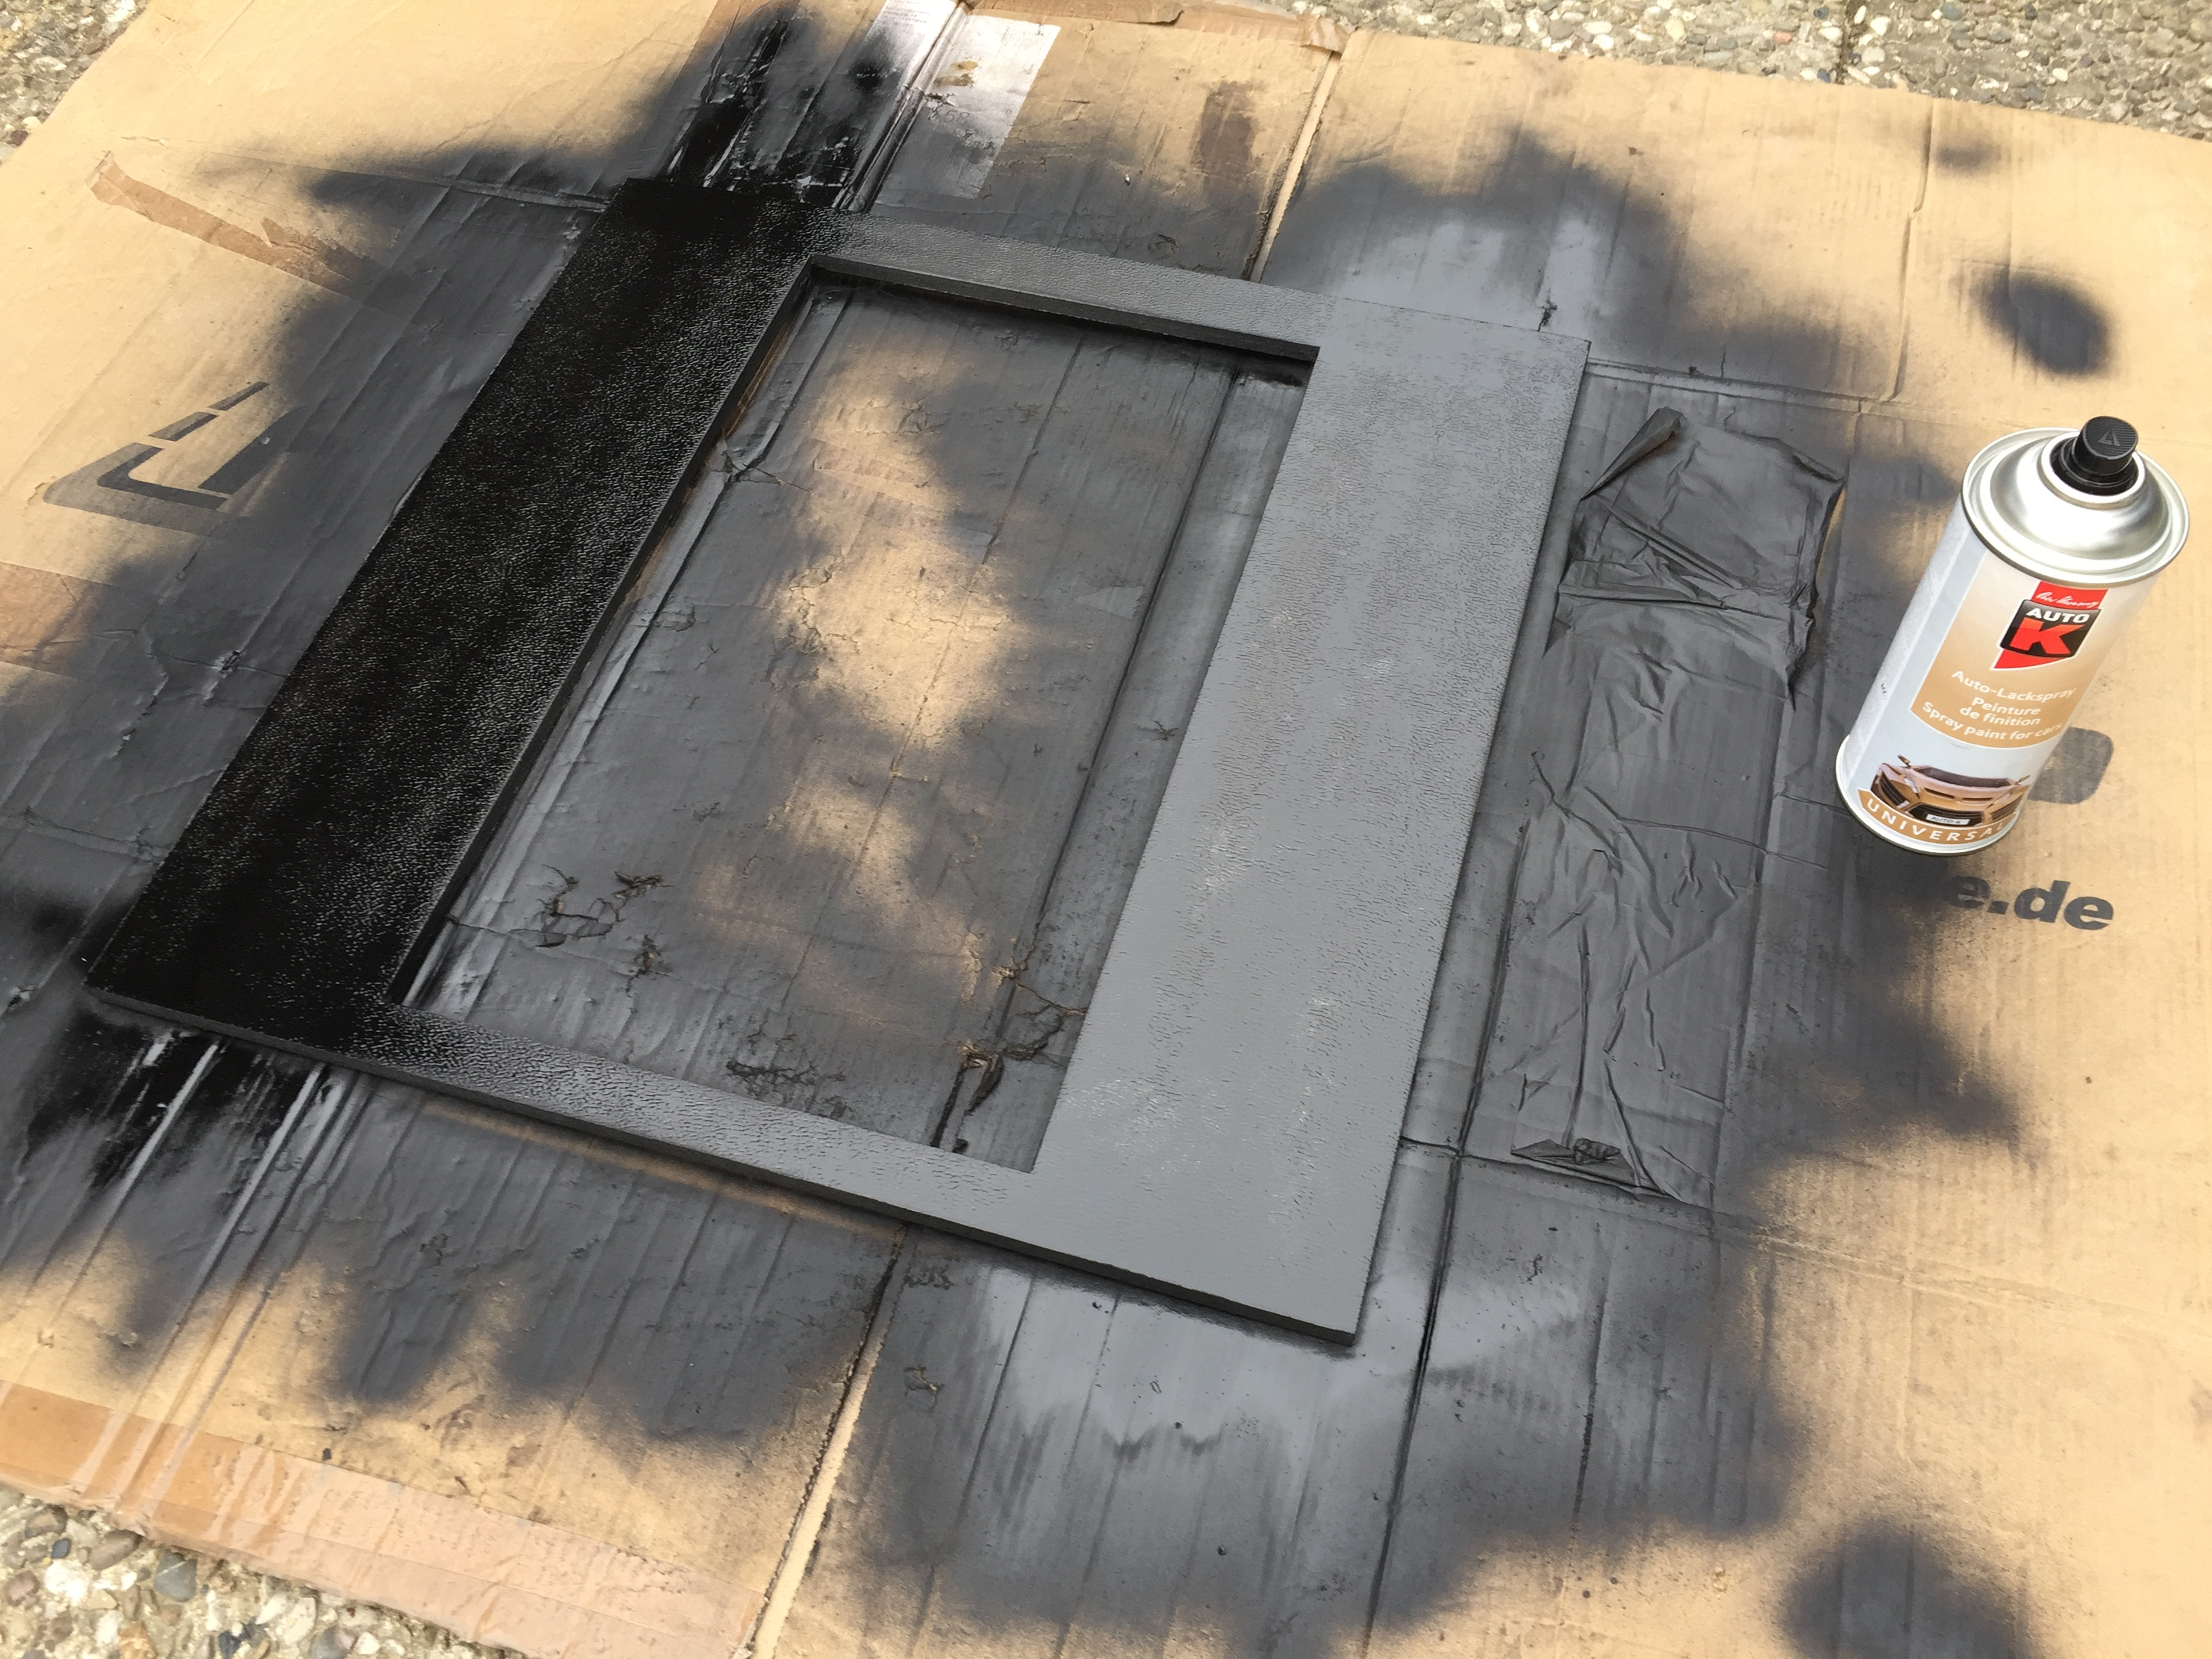
\includegraphics[scale=0.06]{bilder/Hartschaumplatte.jpg}
%	\caption{Lackierung der Hartschaumplatte}
%\end{figure}
%\begin{figure}[H]
%	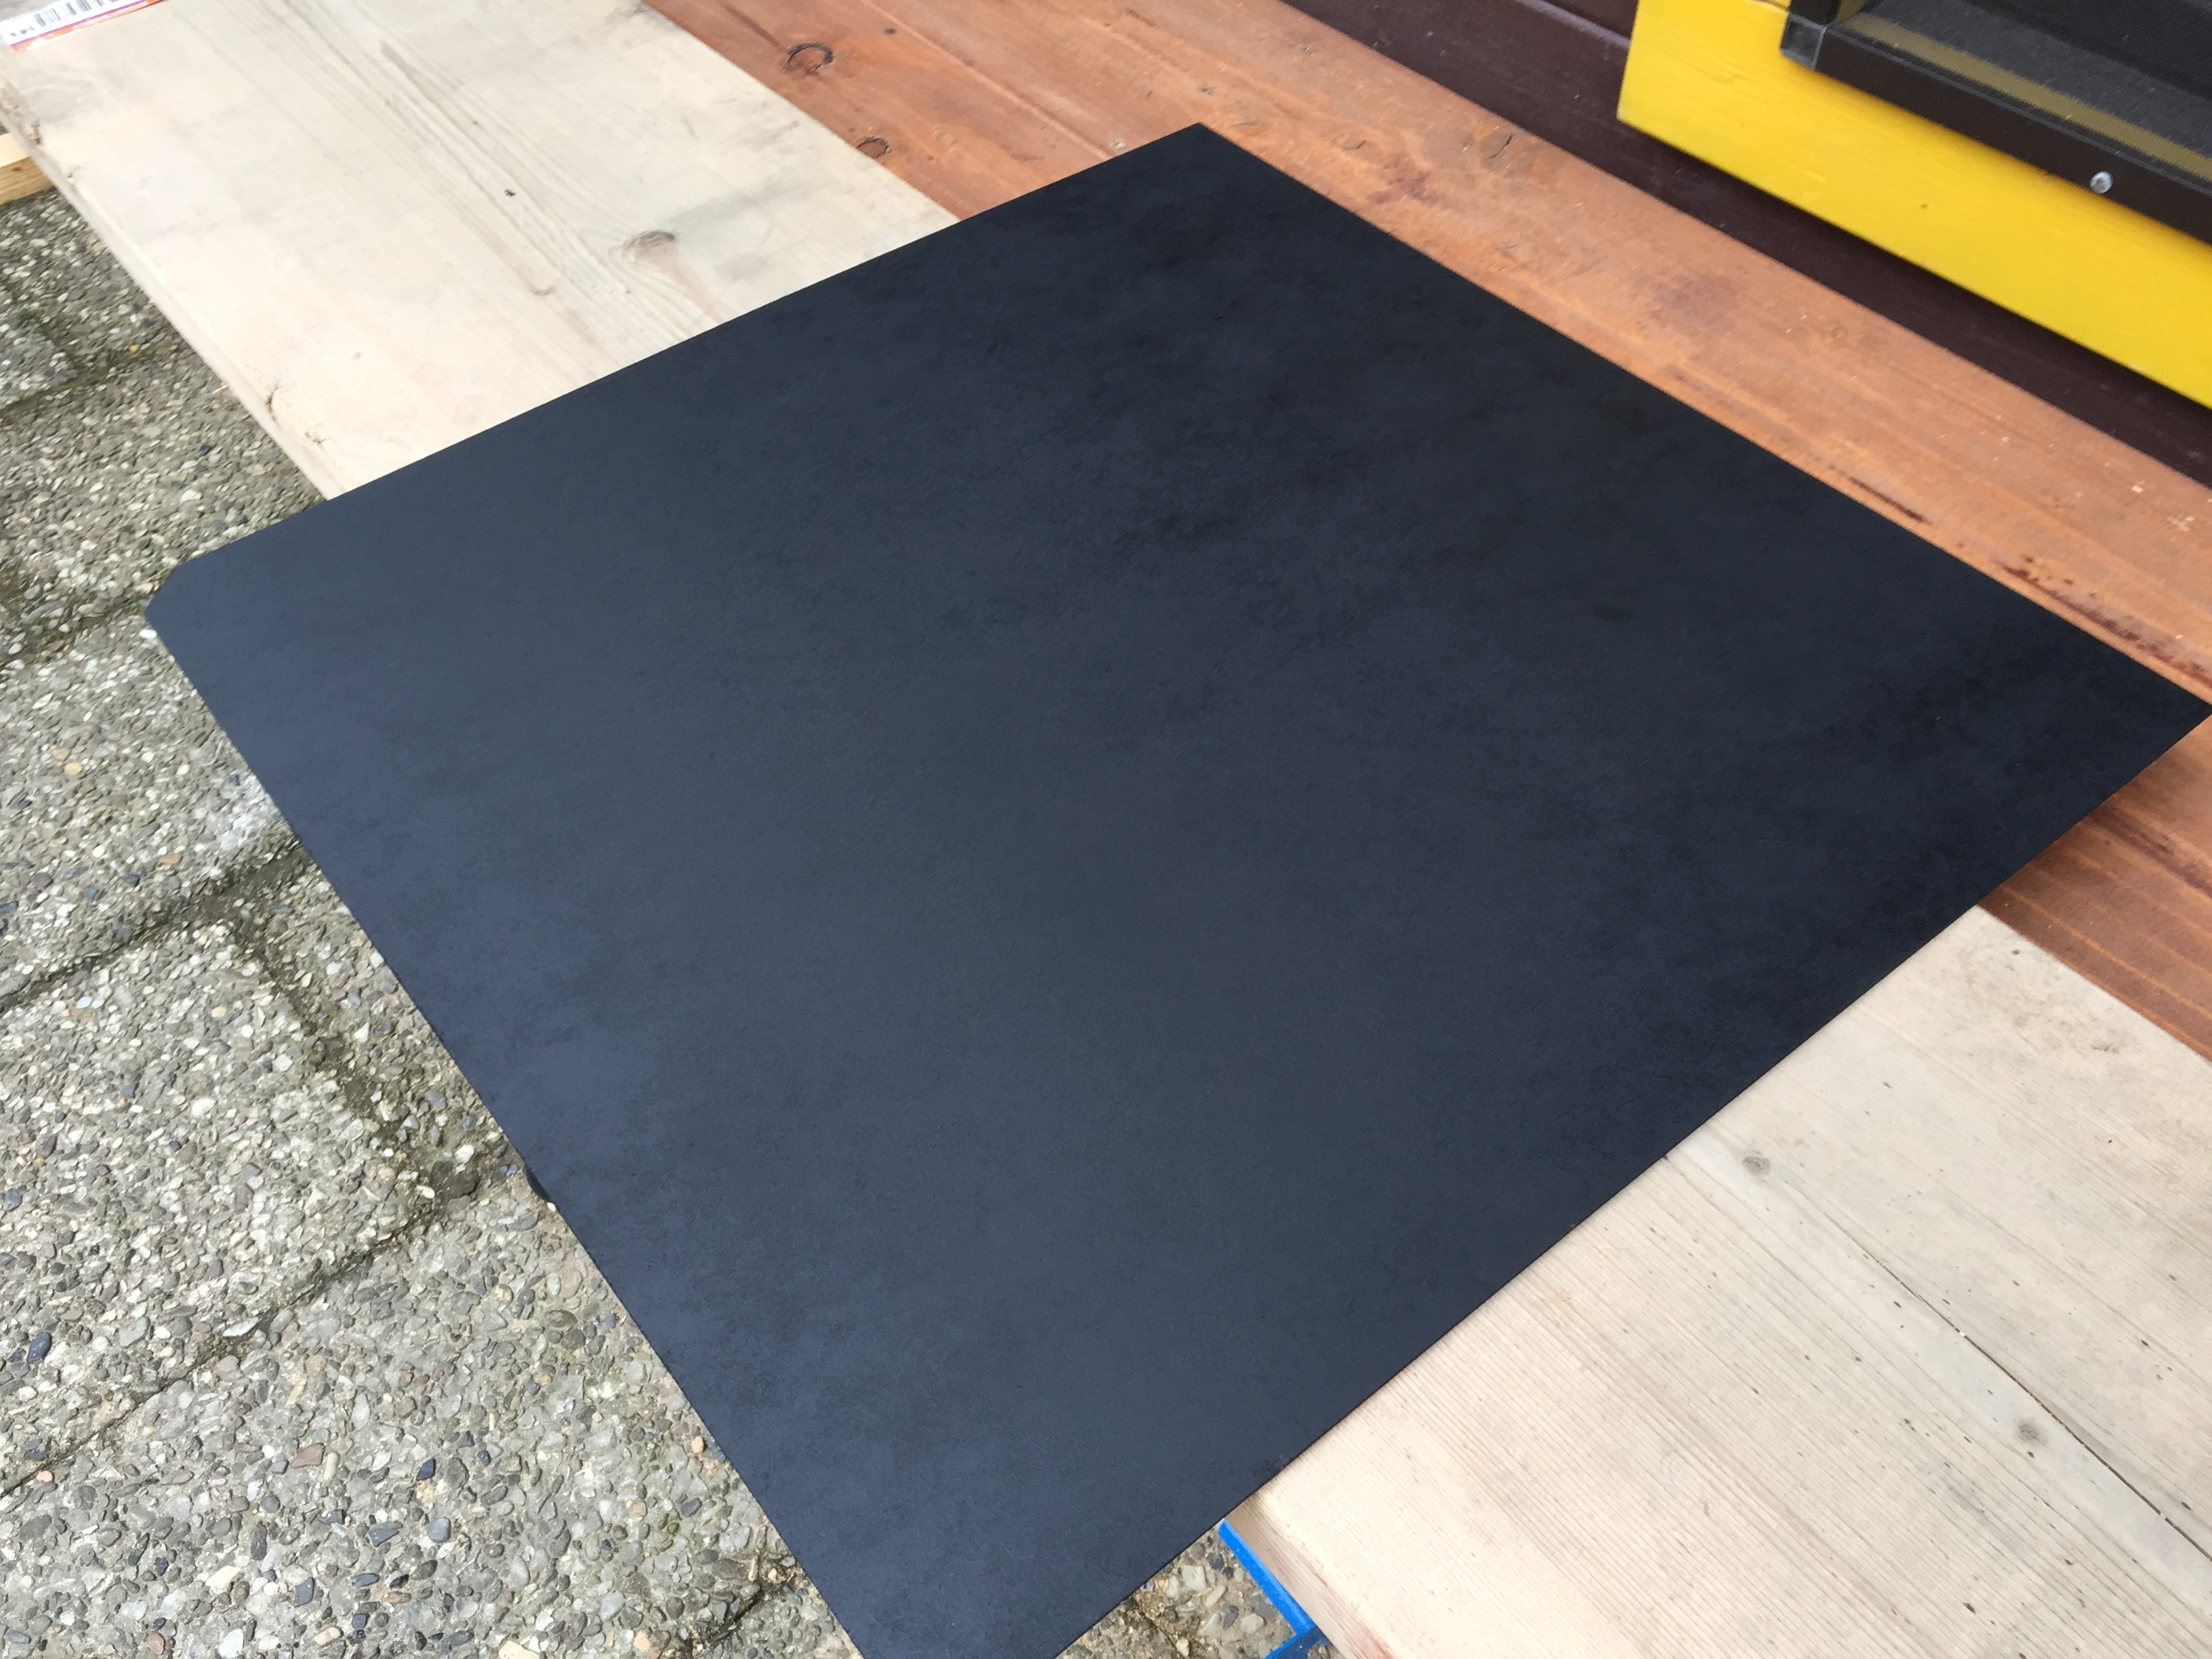
\includegraphics[scale=0.06]{bilder/Rueckwand.jpg}
%	\caption{Lackierung der Rückwand}
%\end{figure}
